\section{Experimental setup}
\label{sec:setup}

\subsection{Data and splits}
We use the interaction-field release of SHOW3D~\cite{rim2026show3d,rim2026show3dapi}: 468 recordings of 10 subjects manipulating 21 objects, captured at 60\,fps by the two monochrome cameras of a Meta Quest~3 headset and released undistorted at $1024\times1280$. Labels for the three official test subjects are withheld and the evaluation server closed on 31~August~2026, so all results are reported on held-out \emph{training} subjects with subject-level splits: fold~A holds out XYZ109 and LYA722, the development split of the organisers' baseline and of GOLF~\cite{zou2026golf}, and fold~B holds out MHA016 and MMO925. No recording appears in both partitions of a fold, the official test subjects are never downloaded, and an automated check verifies both properties before every run. Frames are sampled at 10\,fps for label statistics, matching the organisers' protocol, and every second sampled frame (5\,fps) is used for the token-based models; a frame contributes a target for a hand when headset tracking, the object pose and that hand pose are valid, exactly as in the official label code. Our derived labels reproduce the organisers' count of 87,366 labelled frames at 10\,fps and match the official field to within $10^{-14}$\,mm on the frames we compared. Fold~A trains on 37,645 frames and validates on 5,955 (11,948 at 10\,fps, the exact development split); fold~B trains on 35,052 and validates on 8,548.

\begin{figure*}[t]
\centering
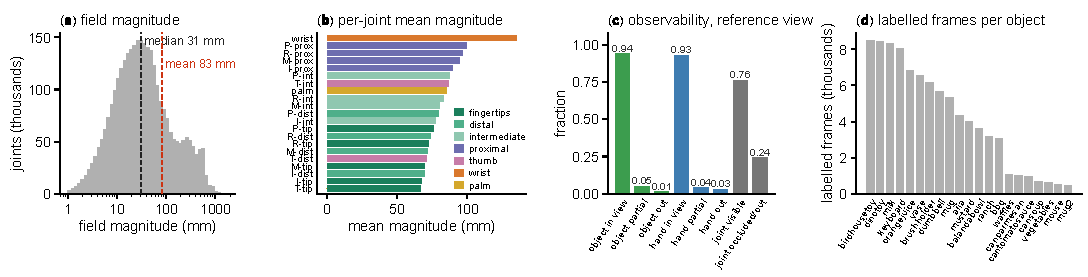
\includegraphics[width=\textwidth]{../figures/fig8_dataset_stats.pdf}
\caption{Statistics of the derived interaction-field labels (10 training subjects at 10\,fps, 87,366 frames, 3.1\,M joint vectors). (a) The magnitude distribution is heavy-tailed: median 31\,mm, mean 83\,mm, 30\% of joints beyond 60\,mm. (b) Mean magnitude per joint: fingertips and distal joints are typically in contact, the wrist is typically far from the object. (c) Observability in the reference view: the object is at least 90\% inside the image in 94\% of labelled frames and essentially out of view in 1.3\%; 24\% of joints are occluded by the object or outside the image, and those joints are mostly in contact (median magnitude 11.8\,mm against 39.8\,mm for visible joints). (d) Labelled frames per object; several objects are handled by one to three subjects only.}
\label{fig:dataset}
\end{figure*}

\subsection{Label statistics}
\Cref{fig:dataset} summarises the derived labels. Of 138,579 sampled frames, 91.2\% have valid headset tracking, 72.2\% a confident object pose and 63.0\% at least one confident hand together with the object, giving 68,270 left-hand and 79,272 right-hand fields; 60,176 frames carry both hands. The joint field is heavy-tailed (median 30.6\,mm, mean 82.8\,mm, 30.2\% of joints beyond 60\,mm) and strongly joint dependent: fingertips have a median magnitude of 13.8\,mm and 52\% lie within 15\,mm of the object, whereas the wrist has a median of 96.5\,mm and 87\% of wrist vectors exceed 60\,mm. Any mean-ADE number is therefore dominated by far-field vectors of the wrist, the proximal joints and non-interacting hands. Joints that the object occludes or that fall outside the image account for 24.0\% of all joints and are mostly in contact (median magnitude 11.8\,mm); the object is out of the reference view in only 1.3\% of labelled frames and hands in 3.0\%, so unobservable targets cannot account for a large share of any model's error, contrary to a hypothesis we held at the outset. The stereo baseline is 63.9\,mm, the focal length 454\,px and the median joint depth 308\,mm (90th percentile 441\,mm), giving a median disparity of 94\,px and a depth resolution of 3.3\,mm per pixel of disparity. Ground-truth hand landmarks carry a median error of 6.4 to 7.9\,mm and object translations of 1.5 to 3.5\,mm according to the dataset authors~\cite{rim2026show3d}.

\subsection{Metrics}
We report the official mean ADE, acc@$\{10,50,100\}\mm$ and recall (always 1.0 for our models, which predict both hands), and geometric measures computed with the ground-truth joints as anchors so that all methods are comparable: the surface distance (SD) from the predicted endpoint $\joint_{h,j}+\hat{\field}_{h,j}$ to the nearest vertex of the ground-truth posed object; the direction error between $\hat{\field}$ and $\field$ for $\|\field\|>20\mm$; the magnitude error $|\|\hat{\field}\|-\|\field\||$; and the decomposition of the endpoint error into its component along the ray from the reference camera through the ground-truth endpoint and the lateral remainder. ADE is further stratified by field magnitude ($<15$, 15 to 60, $>60\mm$), by joint visibility in the reference view (inside the image and not occluded by the object, tested by ray-mesh intersection against the posed mesh), by the fraction of object vertices and of hand joints inside the reference image (at least 90\%, 10 to 90\%, below 10\%), by joint group, hand, object and subject. For factored models we additionally evaluate each head alone and the geometric head with either argument replaced by its ground truth.

\subsection{Baselines}
The baselines are (B1) the official SHOW3D baseline~\cite{rim2026show3dapi}, which carries the InterField name of \cref{sec:related} over to an image-only ResNet-50~\cite{he2016resnet} on the full $224^2$ frame regressing the camera-frame field; we report the organisers' published number on the identical fold-A split rather than retraining it; (B2) a direct joint-query regressor on frozen DINOv3 ViT-B/16 tokens of the reference view; (B3) the same with both views and Pl\"ucker-ray token embeddings, \ie{} the consensus architecture of the challenge solutions~\cite{zou2026golf,jin2026jssr} without backbone adaptation or region sampling; (B3b) B3 with the ray encoding removed; and the zero, training-mean and hand-crop-oracle reference predictors from the starter kit. \method{} adds the geometric head, the auxiliary losses and the precision fusion of \cref{sec:method} on top of B3's tokens; all token models share the encoder, the cache, the decoder width (384), the number of heads (8), the depth ($L{=}6$), the feed-forward width (1536), dropout (0.1), token dropout (0.1), the optimiser (AdamW~\cite{loshchilov2019adamw}, learning rate $2\cdot10^{-4}$, weight decay 0.05, $\beta=(0.9,0.95)$, 300 warm-up steps followed by a cosine schedule), the batch size (32) and early stopping (patience 3 on validation ADE with a minimum improvement of 0.05\,mm), with an epoch budget of 10 that we raise to 30 for the much smaller HOT3D-only runs of \cref{sec:cross}. Nothing was tuned on the held-out subjects beyond this early-stopping rule, which applies identically to every model. The main comparison is repeated with a second seed on fold~A.

\subsection{Implementation}
Tokens are extracted once at $480\times384$ in half precision, projected by principal component analysis to 256 dimensions (the 256 components retain 92.4\% of the variance of 200,000 sampled tokens) and stored as 8-bit integers with per-token scales; the cache of 124,954 images occupies 22\,GB. Object meshes are the binary glTF models bundled with the dataset API; 16 control points and 1,024 vertices per object are farthest-point sampled for the geometric head, while evaluation and label generation use the full meshes. Everything is implemented in PyTorch~\cite{paszke2019pytorch} and runs on a single Apple M5 laptop with 16\,GB of unified memory: feature extraction at 16 images per second, training at 48 samples per second for the stereo factored model and 102 for the single-view direct model, with a peak memory of 5.6\,GB. A full training run takes 1.1 to 2.5\,h and the complete set of experiments in this paper about 35\,h.
